\documentclass[10pt,conference]{IEEEtran} 

\usepackage{latexsym,times}
\usepackage{epsfig}
\usepackage{amsmath}
\usepackage{graphicx,dblfloatfix}
\usepackage{tabularx}
\usepackage{verbatim}
\usepackage{listings}
\usepackage{algorithm}
\usepackage{algpseudocode}
\usepackage{caption}
\usepackage{multirow}
\usepackage{pifont}

%\setlength{\textwidth}{6.5in} \setlength{\textheight}{8.5in}
%\setlength{\columnsep}{2.0pc} \evensidemargin=0in
%\oddsidemargin=0in
%\renewcommand{\textfloatsep}{8pt}
%\topmargin=-0.43in \topskip=0pt
%\renewcommand{\textfraction}{0.0}
%\renewcommand{\topfraction}{1.0}
%\renewcommand{\dbltopfraction}{1.0}

%\def\denseitems{
%\itemsep1pt plus1pt minus1pt
%\parsep0pt plus0pt
%\parskip0pt\topsep0pt}


\newenvironment{smallitem}{
   \setlength{\topsep}{0pt}
   \setlength{\partopsep}{0pt}
   \setlength{\parskip}{0pt}
   \begin{itemize}
   \setlength{\leftmargin}{.2in}
   \setlength{\parsep}{0pt}
   \setlength{\parskip}{0pt}
   \setlength{\itemsep}{0pt}}{\end{itemize}}

\newenvironment{smallenum}{
   \setlength{\topsep}{0pt}
   \setlength{\partopsep}{0pt}
   \setlength{\parskip}{0pt}
   \begin{enumerate}
   \setlength{\leftmargin}{.2in}
   \setlength{\parsep}{0pt}
   \setlength{\parskip}{0pt}
   \setlength{\itemsep}{0pt}}{\end{enumerate}}

\newenvironment{smalldescription}{
   \setlength{\topsep}{0pt}
   \setlength{\partopsep}{0pt}
   \setlength{\parskip}{0pt}
   \begin{description}
   \setlength{\leftmargin}{.2in}
   \setlength{\parsep}{0pt}
   \setlength{\parskip}{0pt}
   \setlength{\itemsep}{0pt}}{\end{description}}

%\newcommand{\comment}[1]{{\sf (#1)}}
\newcommand{\equationstart}{\small
\abovedisplayskip=2pt \belowdisplayskip=2pt
\abovedisplayshortskip=6pt \belowdisplayshortskip=6pt}

\newcommand{\equationend}{\normalsize}

\begin{document}

\input{epsf}

\pagestyle{plain}

 \title{A Collaborative Filtering Recommender System \\ 
for Test Case Prioritization in Web Applications}

%\numberofauthors{2}
\author{\IEEEauthorblockN{Author 1}
	\IEEEauthorblockA{Departemant of ABC\\
		University of x\\
		X, X, X\\
		X@ABC.edu}
	\and
	\IEEEauthorblockN{Author 2}
	\IEEEauthorblockA{Departemant of ABC\\
		University of x\\
		X, X, X\\
		X@ABC.edu}
}

%\author{
%	\alignauthor Author 1\\
%	\affaddr{University of ABC}\\
%	\affaddr{x, y}\\
%	\email{authore1@abc.edu}
%	\and  % use '\and' if you need 'another row' of author names
%	% 4th. author
%	\alignauthor Author 2\\
%	\affaddr{University of ABC}\\
%	\affaddr{x, y}\\
%	\email{authore2@abc.edu}
%}

%\author{
%Maral Azizi \\
%University of North Texas\\
%maralazizi@my.unt.edu
%\and 
%Hyunsook Do \\
%University of North Texas \\
%hyunsook.do@unt.edu
%}

\maketitle
\thispagestyle{empty}


\begin{abstract}
The use of more relevant metrics of software systems could improve
various software engineering tasks, but identifying relationships among
metrics is not simple and can be very time consuming. 
Recommender systems can help with this decision-making process; many applications
have utilized these systems to improve the performance of their applications.
To investigate the potential benefits of recommender systems in regression 
testing, we implemented an item-based collaborative filtering recommender
system that uses user interaction data and application change history 
information to develop a test case prioritization technique.
To evaluate our approach, we performed an empirical study using three 
applications with multiple versions by comparing four control techniques.
Our results indicate that our recommender system can help improve the 
effectiveness of test prioritization; the performance of our approach
was particularly  noteworthy when we were under a time constraint.  
\end{abstract}



%\vspace*{6pt}
\textbf{Keywords: }{Recommender system, test case prioritization, 
regression testing, risk measurement, code quality.}

%\vspace*{12pt}
%
%\baselineskip=18pt

\section{Introduction}
\label{sec:introduction}
% what is the problem?
During application's life it may change several times, and one change can affect the entire system.
To avoid the undesirable change or bugs, system testers need to  
test the overall functionality of the system before deploy the new release of the system.
One of the most common way to evaluate the system quality in sequence of release is regression testing.
In regression testing, testers check the software to ensure that new changes have not 
introduced new faults or it did not effect the other parts of system.
Applying regression testing before deploying new release of the software, make the 
change process safer and more confident for developers.

As software grow, the size of test suite grow in a same
manner, eventually testing the entire system can become expensive and may take
40\% of whole project budget[].  Moreover, it is not feasible to test every single 
function of the system especially for large scale systems it may takes several days 
to execute test cases. Several techniques have been proposed to solve this issue 
%by reducing the cost and effort of system testing.
such as, test reduction which is a 
technique that select subset of test cases that can address most of the issues, 
test selection also is a similar to test reduction but the main difference is 
this technique, select test cases based on their correlation with the changes 
in tow versions of the subject, and test case prioritization [].

% what approaches have been proposed?
Test case prioritization is a technique to catch the faults earlier, 
by executing the most important test cases first.
So far, many prioritization strategies have been proposed by researchers [] and
many techniques have been purposed such as : greedy techniques [], change impact analysis [],
clustering approaches[], user session based techniques [], etc. 
but most of the investigated studies are based on two main features: code coverage and 
code complexity metrics. Meanwhile, there are many other features of the software 
that can be a factor of failure or can be a hint to find the failure causes. 
One interesting feature of web application is that recording users interaction data
is a way easier compare to other types of applications. 
Different types of data from users interaction can be
monitored, such as users sessions, cookies, telemetry data, users IP address etc. 
Storing and collection log files and users sessions nowadays are less costly and more 
accessible compare to past decades, due to lower price of the IT services and hardware.
We can store information in database or cloud system 
rather than log files which was a traditional way to storing system back up. 
Having all these types of data and facilities, enables testers to identify most frequently used
components which impact the system strongly. 
% jeff paper

% why they didint work?
Previous studies shown that change history has more significant role in 
terms of finding faults than code metrics []. 
Although, there are several research have been done about the efficiency of 
change metrics for defect prediction, such as [] but, researchers only focused on 
measuring the causes and effect of the changes in software. 
Moreover, users session and telemetry data 
have been used as a factor for research in software testing. 
For example, Elbaum et al.~\cite{elbaum2005profiling} performed a study on regression 
prioritization focusing prioritization at a product level 
by using telemetry from installations. 
Their work was extended in several domain such as, performance issue detection ~\cite{parsons2007automatic},
bug detection ~\cite{wang2008approach}, reliability testing of rule-based 
systems ~\cite{avritzer1996reliability} and failure reproduction ~\cite{jin2012bugredux}. 
Sampath et al. ~\cite{Sampath2008} applied multiple techniques for prioritizing test cases 
by using user sessions as a factor for their techniques. 


Lets conciser a typical test prioritization based on change history. 
In this scenario, testing is based on executing any component that has been 
changed in new release of software [1-2], % ref: A Comparison of Coverage-Based and Distribution-Based Techniques for Filtering and Prioritizing Test Cases
while this could be a minor change that 
does not have a considerable impact on the entire system, 
such as renaming a function or can be a 
component that is used seldom by users, etc. 
In another scenario, we reorder test cases based on the component frequency, 
meanwhile, there might be no change in this particular component compare to previous version.
For example, generally, core components in a system are mostly used components in the entire system 
while, those components due to their significant role have been tested several times and rarely change. 
Due to above challenges, we belive that current studies in test prioritization 
is neither efficient nor sufficient to address the test priritization problem. 
%We believe that applying multiple factors
%rather than focusing on a specific viewpoint would help improve test case prioritization techniques.

%such as, extracting usage patterns from telemetry data besides analysis of change history. 


% what is your solution and why this work?
In this paper we proposed an item based collaborative filtering recommender system 
for test case prioritization in web application which, uses the telemetry 
data as input for users rating and change history of applications 
as items information. The output of our recommender system is the prioritized test 
cases in a way to obtain the better results in terms of finding faults earlier. 
We applied our recommender system in three open source system and one commercial system.
Our hypothesis is: Combination of various metrics can lead us to design 
more efficient model for fault detection. Our approach focuses on both users 
interaction and change history metrics to detect most risky components, then by 
automating the detection of regression issues, we are reducing the analysis effort for 
test prioritization. Our recommender system, may not locate the regression issue sources 
directly, but it will provide a  list of top potential risky components. 

The main contributions of this study are as follows:
1) Proposing a new hybrid test prioritization technique for web applications domain, 
2) Empirical evaluation of proposed technique and three other control techniques, and
3) Highlighting issues occurred during applying the proposed technique and its limitation 
and guidance to testers upon the results of our study. 

The rest of the paper is organized as follows. In Section 2, we
discuss the approach used in the research as well as formally define
collaborative filtering recommender systems. In Section 3, we detail the empirical study
that we performed. Section 4 provides the results of the study. 
Section 5 discusses the results and the implications of these results, and
Section 7 presents related work. Finally, in Section 8, we provide
conclusions and discuss future work.




%The usage of web application in nowadays is very clear for verity of people 
%from IT expert to someone with minimum knowledge of the Internet. 
%Not only many business are dependent on web applications but also
%web application grow very fast, and number of users of web application are
%growing exponentially, these factor made software engineer to spend 
%more time on deign robust system with minimum failure risk. 
%One small bug can cost so much money and time for the company.
%So far many research have been done to eliminate the risk of
%web applications failure such as test driven development, regression testing, 
%and many more but they are not sufficient neither optimum to detect the faults 
%when it occurs. 
%
%During application life it may change several times, and one change can affect the entire system.
%To avoid the undesirable change or bugs, system testers need to  
%test the overall functionality of the system before deploy the new release of the system.
%But still there might be some issues that can be observe later after deployment.
%One of the most common way to evaluate the system quality is regression testing.
%In regression testing, tester are seeking to find the cause of system failure 
%between old and new versions. Advantage of regression testing is, it make the 
%change process safer and more confident for developers.
%By fast increasing size of software systems, 
%size of test suits grow exponentially as a result, testing the whole system is a time consuming process 
%and can take several days, also it is not feasible to test every function of the system.
%Test case prioritization is 
%a technique to catch the faults earlier, by executing the most important test cases first.
%There are different ways to reorder test cases such as code coverage based, 
%based on frequency of use, based on system architecture and many other statistical technique [xx].
%
%
%Another feature of web applications which made it more popular
%compare to other types of software systems is users monitoring and recording 
%users activity is a way easier and accessible [bryce and others]. 
%% example of ppl who used telemetry
%% and converting usage
%There are different types of data from users interaction can be
%monitored, such as users sessions, cookies, telemetry data, users IP address etc. 
%having all these information has several benefits but to mention the most significant in testing area is that it gives an opportunity to the system tester
%to extract the pattern of most frequently used components of the system so, they can spend more effort 
%of fixing issues of such a components than others.
%
%In this paper we proposed a collaborative filtering recommender system 
%for test case prioritization in web application which, uses the telemetry 
%data as input data of users interaction and change history of applications 
%as items information. The output of our recommender system is the prioritized test 
%cases in a way to obtain the better results in terms of finding faults earlier. 
%We apply our recommender system in three open source system and one commercial system.
%
%The rest of the paper is organized as follows. In Section 2, we
%discuss the approach used in the research as well as formally define
%telemetry fingerprinting. In Section 3, we detail the empirical study
%that we performed. Section 4 provides the results of the study. 
%Section 5 discusses the results and the implications of these results, and
%Section 7 presents related work. Finally, in Section 8, we provide
%conclusions and discuss future work.
%
















\section{Methodology}
\label{sec:method}

To support our regression test generation approach 
for web applications, we have developed PARTE (PHP 
Analysis and Regression Testing Engine).
Figure~\ref{fig:overview} summarizes PARTE's three 
main activities (light green boxes) and how these 
activities are related to each other.
Although we implemented the regression test generation technique
that is applied to PHP web applications, the methodology we apply 
here can easily be applied to other languages by extending the 
front end file conversion functionality.   
When we generate test cases, we considered test paths and input
values that make test paths executable. Another important component 
of test cases is test oracles that verify test results, however, 
in this work, we have not considered test oracles, and we discuss
the limitation of our work related to the test oracle issue in 
Section~\ref{sec:limitations}.

%\begin{figure*}[ht]
\begin{figure*}[!ht]
%\vspace*{-5pt}
\centering
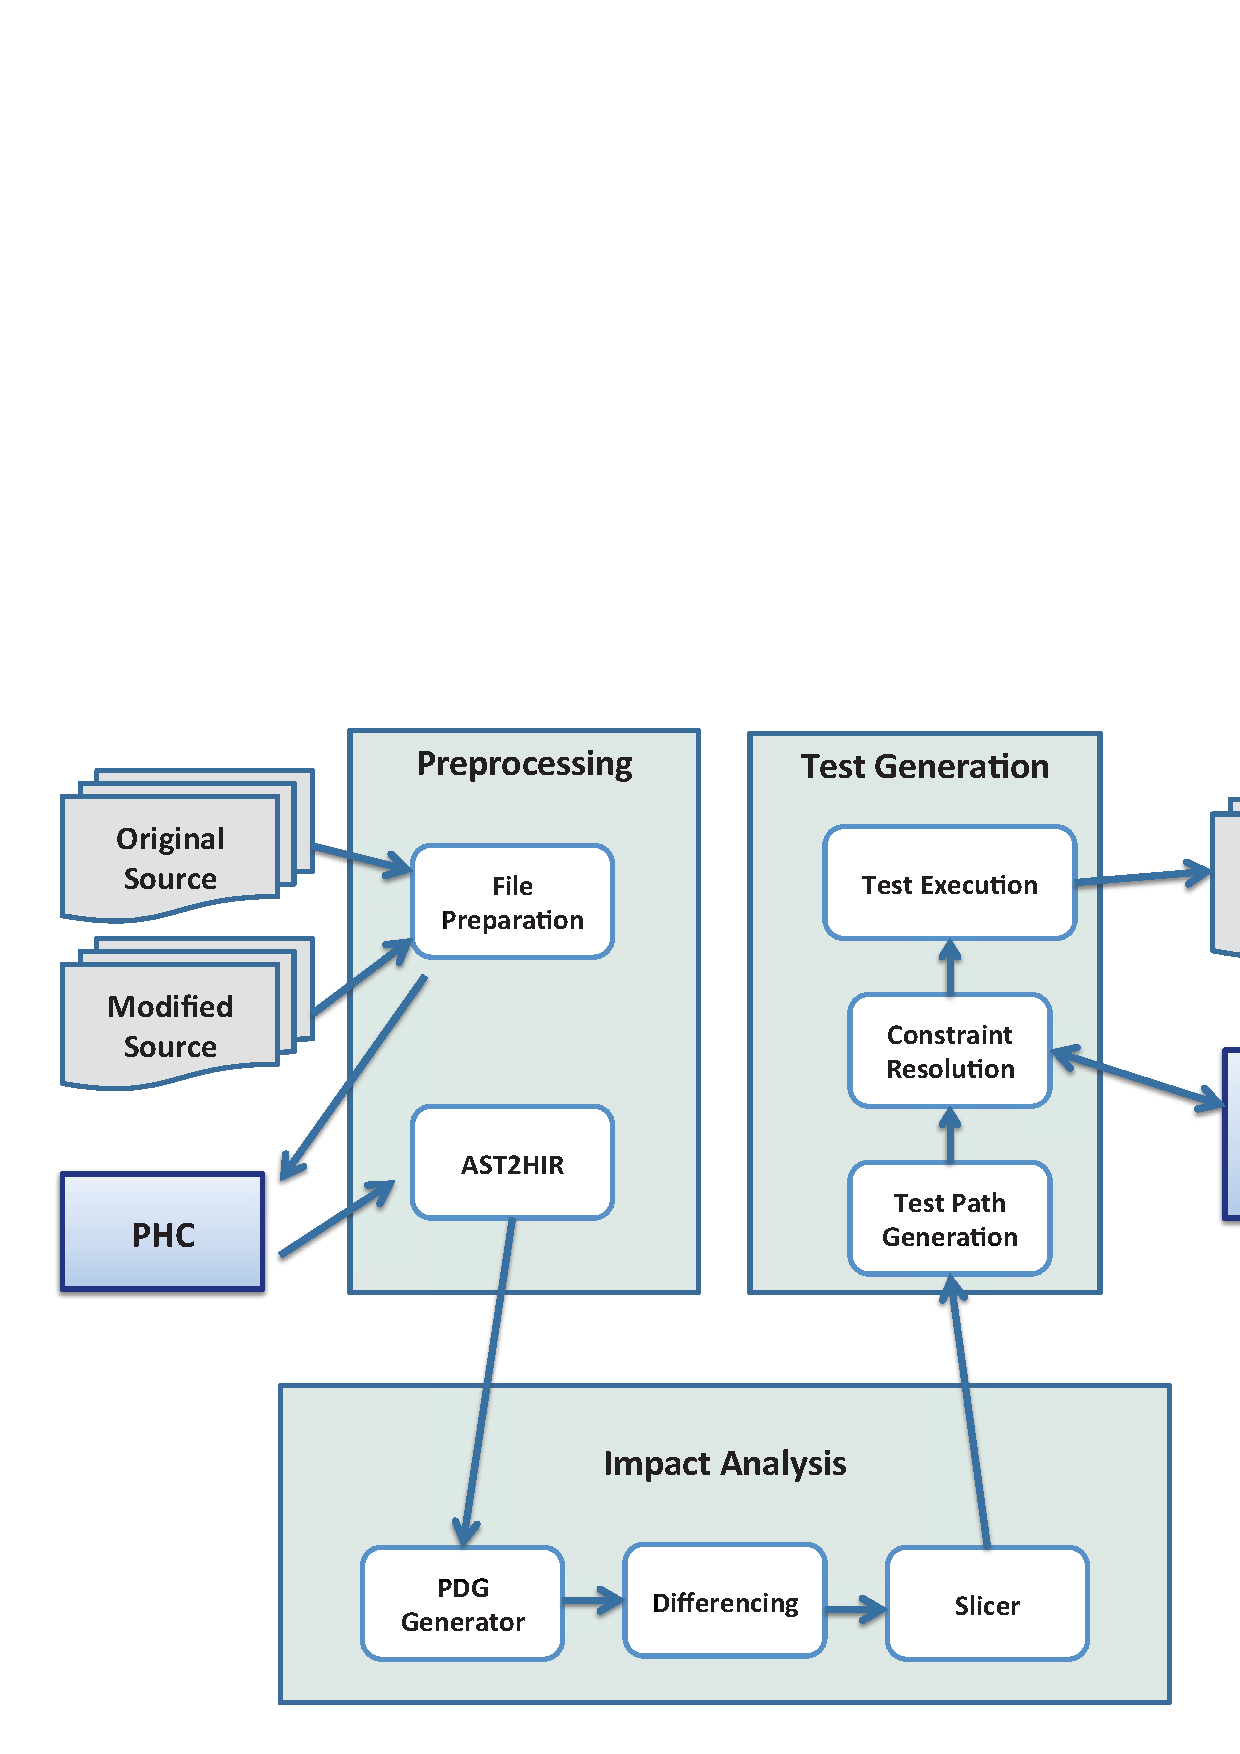
\includegraphics[width=0.8\columnwidth]{figures/parte-overview.pdf}
%    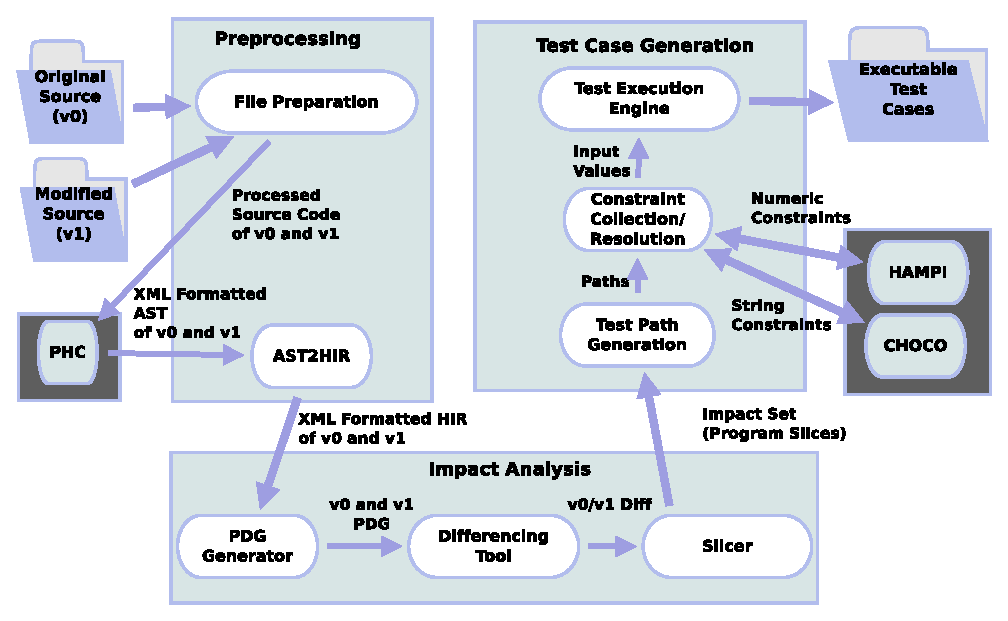
\includegraphics[width=0.8\textwidth]{figures/overview.eps}
\vspace*{-40pt}
 \caption{Overview of PARTE} 
\label{fig:overview}
\end{figure*}

Before we describe each activity in detail,
we provide a brief overview of our approach.

\begin{smallitem}
\item {\bf Preprocessing} (the upper-left box in Figure~\ref{fig:overview}).
In this step, PARTE converts abstract syntax trees (ASTs) generated by
a PHP compiler, PHC~\cite{phc}, to high-level
intermediate representation (HIR) that preserves variable
names and converts this HIR back to ASTs.   

\item {\bf Impact Analysis} (the lower box in Figure~\ref{fig:overview}).
Using preprocessed files, a PDG (Program Dependence Graph) generator 
builds PDGs for the two consecutive versions of a PHP web application. 
Then, a differencing tool and a program slicer identify 
the affected areas by the code changes (program slices).

\item {\bf Test Case Generation} (the upper-right box 
in Figure~\ref{fig:overview}).
A test path generator creates test paths using program slices. 
A constraint collector/resolver gathers string and numeric 
input constraints, and resolves them using a constraint 
solver, Choco~\cite{choco}.
Finally, a test execution engine takes these resolved input 
values, executes the application through Selenium~\cite{selenium},
and records the test execution results.
The last step is done manually because the current path 
generator does not provide web elements for Selenium.
 
\end{smallitem}

\input{ast.tex}
\input{impact.tex}

\subsection{Test Generation}

%\begin{algorithm}[!b]
\vspace*{3pt}
%\begin{algorithm}[ht]
\caption{Path Generation}\label{fig:pathAlgol}
\begin{algorithmic}[1]
{\footnotesize
\State \textbf{Inputs:} \textbf{ \textit{slices[]}} \Comment{\textit{The slices
array contains all of the slices
that are generated by the analyzing changes made to the modified version of the application.}}
\State \textbf{Outputs:} \textbf{\textit{paths}} \Comment{\textit{An array of all of the linearly
independent paths produced from the set of slices.}} 
\State \textbf{Declare:} \textbf{\textit{edges}} \Comment{\textit{A set of edges traveled by the path 
generator}}
\State \textbf{\textit{currentPath}} \Comment {\textit{A placeholder for the path currently being
generator}}
\Procedure{PathGeneration}{$slices$}
	\State $paths \gets \emptyset$ 
	\State $edges \gets \emptyset$ 
	\For{$n \longleftarrow 0 $, $n < slices$.size(), $n$++}
	\While{$slices[n]$.size()$ > 0$}
		\State $currentNode \gets slice[n]$.firstNode()
	    \State $currentPath \gets \emptyset$ 
	    \State $currentPath$.add($currentNode$)
	    \State PDGTraverser($currentPath$, $paths$, $edges$, $slice[n]$, $currentNode$) 
	\EndWhile\label{mainPathWhile}
	\EndFor
	\State ResolvePaths();
	\State \textbf{return} $paths$
	\EndProcedure
}
\end{algorithmic}
\end{algorithm}

%%\begin{algorithm}[htb]
\begin{algorithm}[ht]
\caption{PDG Traverser}
\label{fig:walkpath}
\begin{algorithmic}[1]
{\footnotesize
\Procedure{PDGTraverser}{$currentPath$, $paths$, $edges$, $slice$, $currentNode$}
		
	\While{$currentPath$[lastNode].occursBefore($slice$.endNodes())}
		\If{$currentPath$.containsNoDiffNodes() $\wedge$ $currentPath$.cannotReachAdiffNode()}
		\State	\textbf{Return}
		\EndIf
		\If{$slice[n]$.contains($currentNode$)}
			\State $slice[n]$.remove($currentNode$)
		\EndIf
		\If{$currentPath$[lastNode].getExits.Size() $> 1$}	
			\For {$n \leftarrow currentPath$[lastNode].getExits.Size()-1,0,$n$--}
				\If {$currentNode$.exitEdge($n) \notin  edges$}
					\State $edges$.add($currentNode$.exitEdge($n$)
					\If {$n$ == 0}
						\State $curentNode \longleftarrow currentNode$.exit(n)
						\State $currentPath$.add($currentNode$);
						\State continue(2); \Comment{\textit{Go back to while loop}}
					\EndIf
					\State PDGTraverser($currentPath$.copy(), $paths$, $edges$, $slice$, $currentNode$.exit($n$))
				\Else
					\If{$currentNode$.exitEdge($n$) $\in currentPath$}
					\State $currentNode \longleftarrow$ findFirstNodeOutsideofLoop() 
					\EndIf
				\EndIf
					
			\EndFor 
		\Else
			\State $curentNode \longleftarrow currentNode$.exit(0)
			\State $currentPath$.add($currentNode$);
		\EndIf
	\EndWhile
	\If{$currentPath$[lastNode].isNotASliceEndNode()}
		\If {$currentPath$[lastNode].canReachASliceEndNode()}
			\State $currentPath$.findSliceEndNode();
		\Else
			\State \textbf{Return}
		\EndIf
	\EndIf
	\State $paths$.add($curentPath$)
\EndProcedure
}
%\vspace*{3pt}
\end{algorithmic}
\end{algorithm}

%
%In this phase, we need three steps:
%(1) test path generation, (2) input constraint collection
%and resolution, and (3) test execution.
%The following subsections describe each step in detail.
%  
%\vspace*{3pt}
%\subsubsection{Path Generation}
%
%The path generator creates linearly independent test paths 
%using the slices collected from the previous step.
%A {\em linearly independent path} is a path that includes 
%at least one edge that has not been traversed previously 
%(in a given set of paths under construction)~\cite{pressman}.
%
%Algorithms~\ref{fig:pathAlgol}
%show how to generate test paths using slices. The algorithm 
%is separated into two parts. The first part, 
%Algorithm~\ref{fig:pathAlgol}, iterates through and gathers 
%the nodes from the slice to use in the PDG traversing procedure. 
%The second part, Algorithm~\ref{fig:walkpath}, is the PDG 
%traverser which follows a subpath through the PDG using 
%the nodes in the slice as a guide. Algorithm~\ref{fig:pathAlgol} 
%begins by iterating through every remaining node in each slice.
%
%The PDG traverser (Algorithm~\ref{fig:walkpath}) begins 
%by analyzing a node in the PDG. If the node being 
%processed occurs after every node in the array of 
%remaining slice nodes (line 2), the PDG traverser checks 
%to see if the currently processed node can reach an end node 
%(a node where change propagation terminates) in the original 
%slice (lines 30 and 31). If the node can, it adds the path to 
%an end node of the current path (line 32). Otherwise, the path 
%is discarded (line 33).
%
%If the node that is being processed occurs
%before any of the end nodes in the slice, the node is 
%checked to see if it can reach the changed node (line 3). 
%If it cannot, the path is discarded.
%The PDG traverser then checks to see if a node is
%in the array of slice nodes. If it is, that
%node is removed from the array (lines 6 and 7).
%Every time the PDG traverser encounters a node with more than 
%one edge that has not been traversed, it creates a new subpath 
%that is a copy of itself for each of these edges and follows 
%them (lines 9-18). Once construction of the path has been 
%completed, the path is added to the path array (line 37).
%
%After subpath construction is finished, the first node 
%in a subpath is traced to an entry point for the program, 
%and the last node is traced to an exit point for the program 
%(line 16 of Algorithm~\ref{fig:pathAlgol}). 
%Algorithm~\ref{fig:pathAlgol} describes the basic construction 
%of these paths while omitting, for brevity, all special cases 
%that occur for cyclic graphs (loops and recursion).
%
%\subsubsection{Constraint Gathering and Resolution}
%
%Because the generated test paths contain only input parameters, not 
%actual input values, the input values need to be assigned to the 
%parameters to make test paths executable.
%The constraint collector collects constraints on input
%values needed to execute a particular program execution path.
%Its inputs are the outputs from the PDG generator and path
%generator. The top-level activities in the constraint collector
%are parsing the path and PDG XML files, generating constraints
%for each path, and writing the collected path constraints to
%an XML file. 
%
%Constraint collection begins with path nodes that contain
%a conditional statement. The primary activities to collect
%constraints are determining the truth value of conditional
%statements and reducing the conditional expression in these
%statements. 
%%A constraint is recorded only if it is not
%%a duplicate for a previously recorded constraint.
%A path constraint corresponds to a path PDG node with an
%``if'' statement. To determine the truth value of
%a constraint, the collector looks ahead one node in the
%path node list and examines the node type (which will be
%necessarily either \textit{true} or \textit{false}). After
%determining the constraint truth value, the constraint
%condition is then recursively reduced. Reduction of
%an expression involves parsing the expression string
%to determine the expression type (using regular expression
%matching), creating an expression object with this type,
%assigning any expression attributes from the parsed information
%(e.g., operator type) to the expression object, and generating
%appropriate expression objects for child expressions (if any).
%If there are child expressions, they are recursively reduced
%in the same way.
%
%Each type of expression provides its own method for reducing
%child expressions, in order to take advantage of information
%on the reduction context. For example, a compound boolean
%expression must have child expressions that are themselves
%boolean. When generating child expressions, this information
%can be provided, in addition to that which is provided by
%regular expression matching. This is useful in verifying
%that generated expressions are of the correct type.
%
%If regular expression matching determines an expression
%to be a variable (e.g., \$num\_of\_files), the reduction
%process involves additional steps:
%
%\begin{enumerate}
%  \item The collector backtracks in the path node list,
%starting at the index of the variable node. It continues
%backtracking until a PDG node is encountered that provides
%a definition of the variable, or until the beginning of
%the list is reached. In the case that a definition is found,
%the expression generated for the variable is of the complex
%variable type. This type is used for variables that can be
%defined in terms of other expressions. If, instead, no
%variable definition is found before reaching the start of
%the list, the expression generated is of the simple variable type.
%
%  \item Regular expression matching is performed on the
%variable expression string to determine if it is indexed
%(e.g., \$files[\$id]). These correspond to PHP array variables.
%An expression is then generated for the index of the array, and
%the generated expression for the variable is an indexed version
%of the type determined via backtracking (i.e., simple or complex 
%type).
%\end{enumerate}
%
%The recursive reduction process terminates on expressions of
%simple type, since simple type expressions do not contain
%child expressions that need to be reduced.
%After collecting a constraint, the collector records it for
%inclusion in the output. 
%%This step is only done if an equivalent
%%constraint is not already present in the list in order to
%%avoid outputting duplicate constraints. 
%Once all path constraints
%have been generated, the collector writes the constraint information
%in XML format. 
%
%The tool uses an existing constraint solver, {\em Choco},
%to determine the input values that satisfy the constraints
%for a given execution path (if such satisfaction is feasible).
%{\em Choco} is an open-source software and  consists of a set
%of libraries written in Java that provide many constraint solving
%features. It provides direct support for solving numeric and
%boolean constraints. We also use it to solve string constraints
%by mapping these constraints to equivalent constraints on integers. 
%Once all input values have been created, they are stored in XML file 
%format to be used later by the test execution engine.
%These files contain information about program paths and a list of input 
%variables for the paths. For each input variable, the variable type, 
%name, and value are given. 
%Resolving the inputs that use built-in PHP functions is not supported 
%by our tool, so those inputs require manual resolution. 
%Further, the constraint resolution tool sets the time limit for 
%input resolution, and it reports infeasible when it cannot find 
%the value within the time limit. Also, if the conditions for a 
%variable have conflict, the tool reports that case as infeasible.
%
%\subsubsection{Test Execution}
%
%Having assigned all input values to the parameters in the test 
%paths, we implemented a test execution engine that executes
%test cases over web applications using Selenium~\cite{selenium}.
%We used the Selenium WebDriver API (more specifically, the FirefoxDriver) 
%to set the web page elements according to the variable constraints for 
%the given execution path being tested. If test execution requires setup 
%logic, such as authentication, this is also performed using the WebDriver 
%API. Finally, the WebDriver API is used to execute the PHP file and the 
%results are passed to the test engine.
%As mentioned earlier, web elements are created manually becasue the current 
%path generator does not provide them.
%
%The reason that we have chosen to use the WebDriver API is that it allows us 
%to perform all the activities that will be required: finding and setting web 
%elements; performing any setup tasks required before the test case can be 
%executed (such as authentication); retrieving test execution results in the 
%HTML format.
%
%To give a better understanding of how the approach works, we use an e-commerce 
%example. Assume that we have two PHP files, login.php and add\_card.php, both 
%of which are accessed on different web pages. login.php contains the login 
%form that users can register/authenticate with, and add\_card.php allows 
%authenticated users to add their credit card information. Both login.php 
%and add\_card.php contain entry points for certain execution paths.
%
%If add\_card.php was modified between Version 1 and Version 2, we can run 
%the toolchain on this version pair and determine the constraints necessary 
%to test execution paths with entry points beginning in that file. Using 
%the Selenium WebDriver API, we can first access the login form contained 
%on login.php to register/authenticate the user. Afterwards, we use the 
%same API to directly execute add\_card.php, after initializing the values 
%of the web elements associated with path constraints. It would not be 
%necessary to start from login.php, since the PHP \$\_SESSION variables 
%used for authentication would still be valid during execution of add\_card.php, 
%regardless of the navigational path for arriving at this page. The results 
%of executing add\_card.php are recorded as an HTML file.
%
%
%\input{example-description.tex}



\vspace*{4pt}
\section{Study}
\label{sec:study}

In this study, we investigate whether the use of a recommender system 
can improve the effectiveness of test case prioritization techniques.
We consider the following research questions.

\begin{smallitem}
\item[RQ1:] Can our recommender system be useful for 
improving the effectiveness of test case prioritization techniques?

\item[RQ2:] Can we improve the fault detection rate when we have
only limited budget of time to test the entire system? 
\end{smallitem}

The following subsections present our objects of analysis, 
study setup, threats to validity, and data analysis.

\vspace*{4pt}
\subsection{Objects of Analysis}
\label{sec:objects}

To investigate our research questions, we performed an empirical study 
using two open source applications and one commercial web application.

\textbf{DASCP} is a digital archive and scan software for civil projects; 
 we obtained this application from a private company.  
DASCP is a web based application designed to store civil project 
contracts, which include the technical information of civil and construction projects 
such as project plans and relevant associated information. 
DASCP includes an access control system and provides two types of access rights: 
one user group has permission to edit or insert a project's information or 
upload maps and contract sheets. The other user group is only allowed to view 
the data and details about the projects.

Our second application is \textbf{nopCommerce}, which is a widely-used open 
source e-commerce shopping cart web application with more than 1.8 million 
downloads. This application is written in ASP.Net MVC and uses 
Microsoft SQL Server as a database system ~\cite{nopCommerece}. 

Our last application is \textbf{Coevery}, which is an open source 
customer relationship management (CRM) system written in ASP.Net. 
This application provides an easy framework for users to create their own customized 
modules without having to write any code. The UI design of Coevery has been developed 
by AngularJS and Orchard Technologies~\cite{coevery}. 

\begin{table}
\caption{Subject Applications Properties}
\begin{center}
\begin{tabular}{|l|c|c|c|} \hline
\textbf{Metrics}  & \textbf{DASCP} & \textbf{nopCommerce} 
& \textbf{Coevery} \\\hline \hline
Classes   & 107  & 1,919& 2,258 \\\hline
Files  & 201  & 1,473 & 1,875 \\\hline
Functions & 940  & 21,057 & 13,041 \\\hline
LOC & 35,122 & 226,354 &120,897 \\\hline
Sessions  & 748 & 1310 & 274 \\\hline
Faults  & 35 & 70 & 30\\\hline
Version  & 3 & 23 & 3 \\\hline
Test Cases & 95& 543 & 1,120 \\\hline
Installations & 3 & 2 & 1 \\\hline
\end{tabular}
\end {center}
\label{tab:AUTs}
\end{table}

Table~\ref{tab:AUTs} lists the applications under study and
their associated data: ``Classes'' (the number of class files), 
``Files'' (the number of files), ``Functions'' (the number of 
functions/methods), ``LOC'' (the number of lines of code), 
``Sessions'' (the number of user sessions that we collected), 
``Faults'' (the number of seeded faults), ``Version'' (the number 
of versions), ``Test Cases'' (the number of test cases), and
``Installations'' (the number of different locations where the 
applications were installed). 

Test cases were in application package and we did not implement any 
new test case. Version of open source applications were downloaded 
form the applications' \textit{GitHub} repository and we downloaded all available versions. 


\vspace*{4pt}
\subsection{Variables and Measures}
\label{sec:measures}

\subsubsection{Independent Variable}

To investigate our research questions, we manipulated one independent 
variable: prioritization technique. 
We considered five different test case prioritization techniques,
which we classified into two groups: control and heuristic.
Table~\ref{tab:techniques} summarizes these groups and techniques.
The second column shows prioritization techniques for each group, 
and the third column is a short description of prioritization techniques. 

\begin{table*}[!ht]
\caption{Test Case Prioritization Techniques}
\vspace*{-10pt}
\begin{center}
\begin{tabular}{|l|l|l|}\hline
Group & Technique & Description \\ \hline
\multirow{4}{*}{Control} 
& Change history-based ($T_{ch}$) & Test case prioritization based on change impact analysis score.\\
& Most frequent web forms-based ($T_{mfw}$)&  Test case prioritization based on value of frequency for each web form.\\
& Most frequent methods-based ($T_{mfm}$) &  Test case prioritization based on value of frequency for each method.\\
& Random ($T_{r}$) &  Test execution in random order.\\	
& Greedy ($T_{g}$) &  Test case prioritization in based on code coverage.\\\hline			
\multirow{2}{*}{Heuristic} 
& Hybrid collaborative filtering-based ($T_{hcf}$)& Test case prioritization based on the proposed technique. \\
& Reverse Hybrid collaborative filtering-based ($T_{hcfr}$)& Test case prioritization based on the proposed technique with descending ranking values. \\\hline
\end{tabular}
\end {center}
\label{tab:techniques}
\vspace*{-5pt}
\end{table*}

As shown in Table~\ref{tab:techniques}, we considered four control techniques and 
one heuristic technique. For our heuristic technique, we used the approach 
explained in Section~\ref{sec:approach},
so, here, we only explain the control techniques we applied as follows:

%\vspace*{-5pt}
\subsubsection*{Change History-Based ($T_{ch}$)}
The first control technique is test case prioritization based on change impact
score. In order to perform this technique, we used the information that
we obtained from the change impact analysis approach, which we explained in 
Section ~\ref{CIA-approach}. We prioritized our test cases based on the 
highest scores of the change impact matrix. 
	
%\vspace*{-5pt}
\subsubsection*{Most Frequent Web Forms-Based ($T_{mfw}$)}
This approach determines the web forms that have been most frequently used by users. 
We assume that the most frequently used web forms play a more important role in the system; 
eventually, they should have a higher priority to be tested first. Another reason
why the frequency of web pages is the key for testing is that the most frequently used web pages usually 
contain more functionality and links with other pages, so any bugs on 
those pages can affect greater portion of the entire system. 
Here we define ``base session'' as a long session conducted by our users 
that displays the most interactions in the application.
We picked 20\% of our total sessions as base sessions. 
For example, in online shopping, our base session is a sequence of actions
from user login to checkout, including all necessary actions and some 
random unnecessary actions such as browsing for other items, 
checking the inbox during the shopping process, etc. 
	
\begin{figure}[!ht]
	\centering
	\includegraphics[width=0.90\linewidth]{./SessionSample2.png}
	\vspace*{3pt}
	\caption{Sample of Base Session and Test Sessions}
	\label{fig:sessions}
\vspace*{5pt}
\end{figure}
	
After collecting all sessions, we conducted an analysis of web pages frequency 
by comparing the observed web forms in each session with a base session. 
	
\[
{F_{w,i} = \frac {\sum_{{page\: score\: for \: each\: session}}(S_{i})}
	{\sum_{{number \: of \: base \: sessions}}({BS_{i}})}}	
\]
	
Using Figure ~\ref{fig:sessions} as an example, the page ``PublicStore'' from the base session 
was observed in test sessions 2 and 3. If we assume that we have 
ten test sessions and three base sessions,
and this particular page was observed in seven of the ten pages, then the
frequency of page ``PublicStore'' is equal to $(0.7 / 3) = 0.23$
	
%\vspace*{-5pt}
\subsubsection*{Most Frequent Methods-Based ($T_{mfm}$)}
The most frequent methods approach is nearly identical to the web form frequency technique. 
The only difference is that we considered a method instead of a web form 
as a comparison factor. 
The most frequent methods, usually have high dependency on the other classes and methods. 
If one of them fails, it can cause a significant failure or degradation of the system. 
In order to prevent a domino effect in the system, high frequency methods 
should be tested first, because their failure can cause 
other components failure due to their dependencies.	 	
%Heuristic technique in this study is permuting test cases 
%based on the output list of our	recommender system. 

%\vspace*{-5pt}
\subsubsection*{Random ($T_{r}$)}

Random prioritization selects a test cases in random order.
In this control technique, we randomly selected test cases until
we had executed 100\% of the test cases. \\
	
\subsubsection{Dependent Variable} 

Our dependent variable RQ1 is the average percentage of fault detection (APFD)
referring to the average percentage of faults detected during the test suite execution. 
The range of APFD is from 0 to 100, the higher value indicating better prioritization technique. 
Given $T$ as a test suite with $n$ test cases and $m$ number of faults, 
$F$ as a collection of detected faults by $T$ and
$TF_{i}$ as the first test case that catches the fault $i$, 
we calculate APFD ~\cite{apfd} as follows:

\[
{APFD = 1- \frac {{TF_{1} + TF_{2} + ... + TF_{m}}} {nm} + \frac{1}{2n}}
\]
	
RQ2 seeks to measure the effectiveness of our proposed approach
when we have constrained resources, which means that we need to evaluate 
the effectiveness of our approach using a different metric. 
Qu et al.~\cite{myra} defined the normalized metric of APFD, which is the
area under the curve when the numbers of test cases or faults are not consistent. 
The NAPFD formula is as follows:
	
\[
{NAPFD = p- \frac {{TF_{1} + TF_{2} + ... + TF_{m}}} {nm} + \frac{p}{2n}}
\]
	
In this formula, $n$ is percentage of the test suite run, 
$m$ represents the total number of faults found by all test cases,
$TF_{i}$ indicates the same parameter as AFPF, and 
$p$ is the number of faults detected by percentage of our
budget divided by total number of detected faults when 
running 100\% of test cases.  
	
\subsection{Data Collection and Experimental Setup}
\label{data-collection}
In order to perform our experiment, for both the control and heuristic techniques
we needed to collect three different types of datasets: telemetry data, change 
history, and code coverage information. We explain the data collection processes
in the following subsections.

\subsubsection{Collection of Telemetry Data}
To collect telemetry data, we implemented a small function to record user interactions. 
We considered a sequence of each user's interactions on a specific date as a user session.
First, we uploaded two applications, {\em Coevery} and {\em nopCommerce}, on IIS server 
at the University of ABC in November 2016. 
The server specification is CPU Core i7 with 16 GB of RAM.
After deploying our applications, we recruited volunteer graduate and undergraduate
computer science students and assigned a variety of tasks to them. 
Assigned task to the volunteers were simple scenarios that each application is designed for.
For example, in {\em nopCommerce} we asked them to perform online shopping 
by taking the actual steps which starts from login to payment. We also asked some of 
the users to be the system administrator so we could monitor the whole system 
rather than only the end user side.
We also asked the end users to check the other part of the system randomly like
checking their inbox or wish-list.  
In total, seventy volunteer students performed different tasks during a 40 days period.  
%%% revierw question
In total we collected 1310 and 274 user sessions for {\em nopCommerce} 
and {\em Coevery} respectively. 
%%%%
 
The data collection process for {\em DASCP} is different from that of {\em Coevery} 
and {\em nopCommerce}. {\em DASCP} is a commercial and closed source application 
that has three versions, and it has been installed on the servers of three companies since 2011. 
The DASCP users whose data we examined are real users, and they have application domain knowledge.
We collected twelve-months period of user interactions for DASCP.
As described in Section~\ref{sec:objects}, DASCP provides two types of access rights for users.
In this study, we only considered the sessions of those users who have full access to the system.
In total, 748 user sessions were collected during that period of time. 

%%% more details about sessions
However, the length of the sessions varied by user, date and and workplace.
For example, some users performed all their assigned task few hours before the
determined deadline, while others distributed their tasks into several days.
Average length of user session for {\em nopCommerce} is equal to 56 and for
{\em Coevery} is 24. Although, in some case we obtained sessions length over 
300, specially when the interaction date was close to the deadline. 
Also, most of the {\em Coevery} users are selected from graduate students since the
functionality of this application is relatively more complex than {\em nopCommerce}. 

Figure ~\ref{fig:SampleSession3} shows an example of the raw telemetry data. 
The left column shows the session identifier, which is a user
navigating through the system. The right column is the set of server side user interactions. The structure of the interactions is of the format (Form name):(Control name):(Action name).

\begin{figure}[!ht]
	\centering
	\includegraphics[width=0.90\linewidth]{./SessionSample3.png}
	\vspace*{3pt}
	\caption{Sample User Session}
	\label{fig:SampleSession3}
	\vspace*{5pt}
\end{figure}


\subsubsection{Collection of Code Change History}
We had to take three steps to measure change impact. 
First, we needed a clear understanding of the applications with respect to their changes.
For instance, we needed to check whether a change 
was just the renaming a variable or component, the addition of some comments, 
or an alternation of code by adding or deleting functions, and so on. 
Then, we needed to check whether changes had been made in the current version, 
and finally, we tested a recently changed system~\cite{change3}. 
In order to collect change history information for training, 
we used all versions of our applications.

In our study, we collected the change history of our three applications. 
We chose ten metrics that have high correlations with bugs.
Most of these metrics have been used in bug detection research, and they
are known to be good indicators for locating bugs~\cite{sungmicro, shihab12, 
raimund, change1, change2}.
Table~\ref{tab:historyMetrics} shows the applied change metrics in this study. 

\begin{table}[!ht]
\caption{Change metrics used to evaluate risk in this study}	
\vspace*{3pt}
%\begin{tabular*} {.8\linewidth}{@{\extracolsep{\fill}}l|l|}
\begin{tabular} {|l|l|} \hline
	\textbf{Metrics Name} & \textbf{Description} \\\hline \hline
	Revision & Number of revision of a component  \\\hline
	LOC Added&   Added lines of code \\\hline
	Max LOC Added  & Maximum added lines of code \\\hline
	AVE LOC Added  & Average added lines of code \\\hline
	LOC Deleted  & Deleted lines of code  \\\hline
	Max LOC Deleted & Maximum deleted line\\\hline
	AVE LOC Deleted & Average deleted lines of code \\\hline
	Code Churn & Sum of change in all revisions \\\hline
	Max Code Churn & Maximum code churn for all revisions \\\hline
	AVE Code Churn & Average code churn per revisions \\\hline
	Age & \parbox[t]{5cm}{Age of a component \\ in days from last release} \\\hline
	Time & \parbox[t]{5cm} {Time of a change \\ in dd-mm-yyyy format} \\\hline		
\end{tabular}
\label{tab:historyMetrics}
\end{table}

\subsubsection{Collect Code Coverage}
\label{codecoverage}
Once our recommender system was designed and implemented, 
we needed to find test cases that covered the recommended components. 
We collected the code coverage data for our test cases using code coverage analysis tool  
that Microsoft Visual Studio provides as part of its framework. 
After collecting the code coverage information, 
we entered that information into a relational database. We assigned unique
identifier values for each method and test case which provides
a key for method and test tables. So we could easily map the methods
to the test cases that exercise them.  

 
\begin{table}[!ht]
\caption{Code Coverage Data Table}
%\vspace*{-10pt}
\begin{center}
\begin{tabular}{|c|c|c|c|c|c|} \hline
	MethodID  & Risk Score & TestID1 & ... & TestID n \\\hline
	12 & 0.876 & 0 &  & 0 \\\hline
	287 & 0.012 & 1 &  & 0 \\\hline
	301 & 0.547 & 0 &  & 0 \\\hline
	148 & 0.145 & 0 &  & 1 \\\hline
	67 & 0.055 & 1 &  & 0 \\\hline			
\end{tabular}
\end {center}
\label{tab:coverage}
%\vspace*{-15pt}
\end{table}

	
Table~\ref{tab:coverage} show the code coverage data we collected.
%In our database system these columns are in separate tables and we join them
%by module identifier but to save the space here, we represent them as one table.   
The first column, ``MethodID'', shows
the unique identifier values that we assigned for each method. 
The second column shows the final risk scores, which is the output of 
our recommender system. Other columns list our test cases
with Boolean values: 0 indicates that the test case does not cover 
the method, and 1 indicates that the test case covers the method.

\subsubsection{Seeded Faults}
\label{faultsInfo}
As mentioned in ~\ref{}, faults were seeded manually by graduate students. 
We tried to simulate the naturally developer faults into the applications. 
All seeded faults are in server-side code level and we ignored HTML-based and GUI faults. 
Four types of faults were seeded into the applications. 
First type is data faults, which are faults that related to the interacting with the data store. 
Logic faults that are logic error in code, action faults that modifies parameter values and actions, 
and finally, linkage faults that change the hyperlinks references.  



Once the change history data is collected, we applied 
ANOVA analysis to our dataset to obtain a linear model.
Our goal was to find the correlation coefficient for each 
metric to measure statistical relationships between 
a variable and real defects. The value of this measure 
fluctuates between 1 and -1, where 1 indicates a strong 
positive relationship, 0 indicates no correlation, and 
negative value means reverse correlation.
For example, if we have a -0.87 correlation coefficient score for 
$Age$ metric that indicates that the oldest components of the system
has a less risk of regression faults.   
We also calculated root mean squared error and mean absolute error. 
A lower error value shows that the model has higher prediction accuracy. 
 

In order to evaluate our linear model, we applied 10-fold cross validation. 
By applying linear regression, we obtained a model that determines the weight 
of each variable. In next step we applied our obtained model  
to evaluate the risk score of each component. 
Finally, by having a matrix of components and their relevant risk scores, 
we permuted the test cases. For example, suppose we have five components
$C =\{c_1, c_2, ... , c_5\}$ with risk score 
as follows :   $R =\{0.0014, 0.251, 0.034 , 0.561, 0.138\}$.
Also, suppose we have a list of test cases with their code coverage information.
Then, we will reorder the test cases in such a way to test $c_4$ first, 
since it has highest risk score (0.561), and $c_1$ will be the last 
component to be tested. 

After collecting all the required data, we ran control and heuristic 
techniques and calculated APFD and NAPFD values for the reordered test cases 
to determine whether the proposed technique improved the fault detection rate. 



\subsection{Data and Analysis}
\label{sec:data1}

In this section, we present the results of our experiment
and data analyses.
We discuss further implications of the data
and results for the experiment in Section~\ref{sec:discussion}.

\begin{table}[ht]
\caption{\small Results for Path Generation}
{\small
\begin{center}
\begin{tabular}{|l|c||c|c|c|c|}
\hline
Application & Version Pair & Number of Paths & Number of Paths & Inputs & Reduction \\
 &   & for Entire Application & Generated & Required for & Rate\\
 &   & (path-entire) & by PARTE & path-parte & (path-parte over \\
 &   &  & (path-parte) &  & path-entire) \\
\hline\hline
{\em FAQForge} &  1.3.0 \& 1.3.1 & 73 & 5 & 25 & 93\% \\ \hline
&   1.3.1 \& 1.3.2 & 73 & 19 & 210 & 74\% \\
\hline \hline
{\em osCommerce} &2.2MS1 \& 2.2MS2 & 2403 & 1719 &4392 & 28\%\\ \hline
&2.2MS2 \& 2.2MS2-060817 & 2409 & 58 & 813 & 98\%   \\ \hline
\hline
{\em phpScheduleIt} &  1.0.0 \& 1.1.0 & 481& 338 & 2389 & 30\% \\
\hline
&   1.1.0 \& 1.2.0 & 518& 314 & 3877 & 39\% \\
\hline
&   1.2.0 \& 1.2.12 & 529& 154 & 2339 & 71\% \\
\hline \hline
{\em Mambo} &4.5.5 \& 4.5.6 & 1357 & 65 &490 & 95\% \\
\hline
&4.5.6 \& 4.6.1 & 1388& 1388& 4446 & 0\%  \\
\hline
&4.6.1 \& 4.6.2 & 1416 & 236 & 2075 & 83\%  \\
\hline
&4.6.2 \& 4.6.3 & 1409 & 92 & 1236 & 93\%  \\
\hline
&4.6.3 \& 4.6.4 & 1444 & 114 & 1567 & 92\%  \\
\hline
&4.6.4 \& 4.6.5 & 1444 & 20 & 324 & 99\%  \\
\hline \hline
{\em Mantis} &1.1.6 \& 1.1.7 & 3482 & 221 &1524 & 94\% \\
\hline
&1.1.7 \& 1.1.8 & 3482 & 185 & 1238 & 95\% \\
\hline
&1.1.8 \& 1.2.0 & 4345 & 2802 & 20425 & 36\% \\
\hline
&1.2.0 \& 1.2.1& 4373 & 166 & 1772 & 96\% \\
\hline
&1.2.1 \& 1.2.2 & 4389 & 106 & 1042 & 98\% \\
\hline
&1.2.2 \& 1.2.3 & 4403 & 103 & 890 & 98\% \\
\hline
&1.2.3 \& 1.2.4 & 4419& 199 & 2643 & 95\% \\
\hline

\end{tabular}
\end{center}
\label{tab:results}
}
\end{table}

Table \ref{tab:results}\footnote{There were
a few bugs in the implementation of the path generation algorithm
in our previous work which were fixed before collecting data
for this study. Due to this reason, the data values presented
in this paper do not match those published in our previous
work~\cite{marback12}.} summarizes the data gathered from
our experiment running on {\em FAQForge}, {\em osCommerce},
{\em phpScheduleIt}, {\em Mambo}, and {\em Mantis}.
The table lists, for each application, ``Version Pair''
(two versions of the applications analyzed), ``Number of Paths
for Entire Application (path-entire)'' (the total number of 
linearly independent paths for the latter version), ``Number 
of Paths Generated by PARTE (path-parte)'' (the number of 
linearly independent paths generated using program slices 
for the latter version), ``Inputs Required for path-parte'' 
(the number of input values required for executable test paths),
and ``Reduction Rate'' (test path reduction rate for our approach
(path-parte) over the control technique (path-entire)). 
The number of inputs presented in the table is the summation for
the number of inputs required for each path, thus redundant inputs 
may exist. 

When we consider the entire application for test path generation,
for the latest version of {\em FAQForge}, 73 test paths were 
generated; in the case of {\em osCommerce}, 2409 test paths 
were generated; for {\em phpScheduleIt}, there were 529 test paths; 
{\em Mambo} ahd 1444 test paths; and for {\em Mantis}, 4419 test 
paths were generated. As expected, the number of paths is proportional 
to the size of each application. When we generated test paths by 
applying our approach (path-parte), on average, the test path 
reduction rates over path-entire for the five applications were 
84\%, 63\%, 46\%, 77\%, and 87\%, respectively (in the 
order the applications appeared in the table). 
The following subsections present data analysis for each application.
 
\subsubsection{Results for FAQForge}

For {\em FAQForge}, our test path generator created 5 and 19 
paths for the two pairs of versions, respectively, while the control
technique produced 73 paths for both versions. 
For {\em FAQForge}, the size of the application is relatively small 
compared to other applications, and the changes between versions 
are also very small; therefore, the number of test paths required 
for the new version is relatively small.

Upon manual inspection of the source for the first pair (versions 1.3.0 
and 1.3.1), we discovered that only one of the files in version 1.3.1 
had been changed from version 1.3.0. The modified file was 
a library file that contained functions included by the main index file. 
During path generation, we did not analyze any of the library files 
directly. Instead, the path generator analyzed files that the user 
would execute directly. If {\em FAQForge} files
were not executed directly, they were located in the ``lib'' directory.
Changes made to the library file were propagated to the index file 
during the file preparation phase of preprocessing. 

The second pair for {\em FAQForge} (versions 1.3.1 and 1.3.2) yielded
19 paths using the path generator. Upon manual inspection of the source 
code, unlike the first version pair, it had many changes in the
source files; we found that 12 files in version 1.3.2 had changed from 
version 1.3.1.  Among these 12 files, only three were analyzed directly. 
The rest of files were, again, library files (in the ``lib'' directory)
invoked using the \textit{include} and \textit{require} functions.

As shown in Table~\ref{tab:results}, our technique produced a 
relatively small number of test paths compared to the control technique. 
Our technique reduced the number of test paths by 93\% and 74\% 
for versions 1.3.1 and 1.3.2, respectively. 
The number of inputs required for path-parte for {\em FAQForge}
was small compared to other applications; for each version pair,
the number of inputs was 25 and 210, respectively.

\vspace*{-2pt}
\subsubsection{Results for osCommerce}
\vspace*{-2pt}

For {\em osCommerce}, the test path generator created 1719 and 58
paths for the two pairs of versions, respectively. 
Upon manual inspection of the source for the first pair (versions 2.2MS1 
and 2.2MS2), we found that 279 of the 506 files had changed. 
The modified files were in every module of the application, and the files 
with the largest differences were the library files that were included in 
the executable files. Again, during path generation, we did not analyze 
any library files (files in {\em osCommerce}'s ``include'' directory)
directly. Instead, the path generator only analyzed files that the user 
would execute directly. 

The second pair for {\em osCommerce} (versions 2.2MS2 and 2.2MS2-060817) 
yielded 58 paths using the path generator. Upon manual inspection of 
the source code,  we found that 105 of the 502 files had changed. 
The number of changed files was smaller than the first version pair.
Considering the number of files that were changed for the second version
pair (105 of 502 files), the number of paths generated was relatively 
small (58). The reason was that there were numerous changes in statements 
that contained no variables, and therefore, there were no data 
dependencies. 

As shown in Table~\ref{tab:results}, our technique produced a relatively 
small number of test paths compared to the control technique. 
Our technique reduced the number of test paths by 28\% and 98\% 
for versions 2.2MS2 and 2.2MS2-060817, respectively. 
The input numbers were proportional to the test path number, so
similar to the test path generation results, the number of inputs
required for the version pairs was quite different: 4392 for the first
version pair and 813 for the second version pair.
However, when we consider the ratio between input numbers and test path 
numbers, the first version required a relatively small number of inputs
per path. This result can be attributed to many changes in a simple output 
statement that has no data dependencies. A common example in PHP would 
be to \textit{echo} or \textit{print} static HTML statements.
If the static text changed, we marked the statement as a difference.

\subsubsection{Results for phpScheduleIt}

In the case of {\em phpScheduleIt}, overall,
the test path reduction rates achieved by applying our approach
were low compared to those of other object programs.
In particular, the first two version pairs produced 30\% and 39\%
reduction rates, respectively.
Upon manual inspection of the source code for the first two version
pairs, we found that they involved large functionality 
changes and bug fixes. For the first version pair, among 90 files, 
71 files were changed between the pair. For the second version pair, 
among 143 files, 105 files were changed. 
Due to these extensive changes among files, many code
components needed to be tested, and this was the major reason
for the low test path reduction rates.

For the last version pair, the reduction rate was 71\%, which 
was better than the previous version pairs, but it was slightly 
low compared to other applications.
Our manual inspection found that, among 178 files, 139 files were changed.
While the number of modified files was similar to the second version
pair, the files that contained a large number of code involved minor changes,
so the affected code area was not large; as a consequence, the test path 
reduction rate was higher than other version pairs.
The number of inputs required for path-parte for each version pair
was 2389, 3877, and 2339, respectively.

\subsubsection{Results for Mambo}

For {\em Mambo}, the test path reduction rates for all version pairs
but one were high, ranging from 0\% to 99\%. In particular,
for the last version pair, the reduction rate achieved by applying
our approach was 99\%. This fact indicated that less than 1\%
of test cases are actually required for the modified web application,
a huge savings considering the application. (Note
that the size of the last version of {\em Mambo} is over 133 KLOC.)

Our manual inspection showed that a few minor changes were
introduced between those versions (e.g., 4.6.4 and 4.6.5). Only 14 files
were changed among the 663 files for the version pair. As a result, only
20 test paths were needed for the new version.
Version pair 4.5.5 and 4.5.6 also produced a high reduction rate.
We found that 319 files were changed among the 703 files for this version 
pair, so a high reduction rate was unlikely. Further inspection of 
the source code revealed that most changes were not in the code 
part but in the top comment section for the disclaimer. Thus, these changes
did not affect the number of test paths required for version 4.5.6. 

Unlike other version pairs, for 4.5.6 and 4.6.1, we did not gain any
benefits by applying our technique. By looking at their version number 
changes, we can infer that there were major changes between these 
two versions. In fact, version 4.5.6 was released on 22 Jan 2008, and 
the next version (4.6.1) was released after 10 months (04 Oct 2008), which
indicated that there was a major change between these two versions.
Upon manual inspection of two versions, we also found that a large 
area of code had been changed. Among the 719 files, 317 files were changed, 
and most of the changes were extensive in nature. Most of the functions 
were changed as part of refactoring and the feature update.
These changes required to generate test paths for the entire application.
As a result, a large number of inputs (4446) was also required for those 
test paths. 

\subsubsection{Results for Mantis}

Similar to the {\em Mambo} results, the test path reduction rates
for {\em Mantis} were very high with one exception (the version pair
1.1.8 and 1.2.0). The rates ranged from 36\% to 98\%, and except 
for the third version pair, our approach achieved over 90\% of 
the reduction rate. For these version pairs that produced over 90\% 
of the reduction rate, we found minor functionality changes and bug 
fixes in the source code. There were no big changes in any module of 
the source code. We also inspected the version pair 1.1.7 and 1.1.8
which produced 95\% reduction rate. There were only four minor bug 
fixes and one translational update.  Version 1.1.8 was intended for 
wrapping up minor things before developing the next major release, 1.2.0.

For only one version pair (1.1.8 and 1.2.0), the reduction rate (36\%) 
was low. By inspecting the release date and release notes 
for this version pair, we found that it was a major release
which included large functionality improvement, a large number of bug fixes, 
and architectural restructuring. Manual inspection of the source code also 
reaffirmed the extensive changes. Among the 496 files, 260 files were changed.
For these reasons, almost all components in the modified version needed 
to be tested.


\section{Discussion}
\label{sec:discussion}

To further explore the results of our
experiment, we consider three issues:
(1) a summary of the test path generation results
obtained in this experiment and the practical implications,
(2) a discussion of test input constraints, 
and (3) a discussion of the security implications for our approach.
Following this discussion, we address the limitations of our work. 

\subsection{Test Path Generation Results and Practical Implications}

Our results from the experiment strongly support the conclusion 
that the program slice based test case generation approach needs 
fewer test cases to test the modified version of the program 
compared to the control technique.

To show our results visually, we present them in bar graphs as shown
in Figure~\ref{fig:bargraph}. The figure contains five subfigures 
that present results for each object program, and each subfigure 
contains bar graphs that show the total number of test paths produced 
by two techniques (control (path-entire) and our technique (path-parte)).

As the figure shows, for all version pairs of all object programs, 
our approach generated a smaller number of test paths than the control 
technique, and for the majority of the cases, the difference between 
the control technique and our approach was very large. 
In total, 12 of 20 version pairs produced over a 90\% reduction rate, for
{\em Mambo} and {\em Mantis}, all cases but two produced substantial 
reduction rates. 
However, for some cases, the difference between these approaches was not 
outstanding. For instance, with the first version pair in {\em osCommerce}, 
the first two version pairs in {\em phpScheduleIt}, the second version pair 
in {\em Mambo}, and the third version pair in {\em Mantis}, 
the savings produced by our approach were smaller than average.
We speculated that the version release affected this outcome. 
When a software system goes through major version changes, 
more functionalities tend to be added, and code refactoring can take 
place; therefore, more code modifications are involved for the major revisions
than for small bug fixes or feature updates.
In fact, the version pairs that did not produce huge savings went through
major changes, and large portions of code were refactored.

The version pairs that produced substantial savings indeed involved
minor bug fixes and small feature upgrades. 
This is the exact situation where we aim to apply our approach
as we described in the Introduction section. 
Revisions caused by bug fixes or security problems tend to be unexpected 
and unplanned compared to major revisions, thus a short turnaround time 
for releasing these revisions is a dire issue. By providing regression testing 
approaches that can save time and effort, we help deploy the applications
as early as possible.

\begin{figure*}[ht]
%%\vspace*{-12pt}
\centering
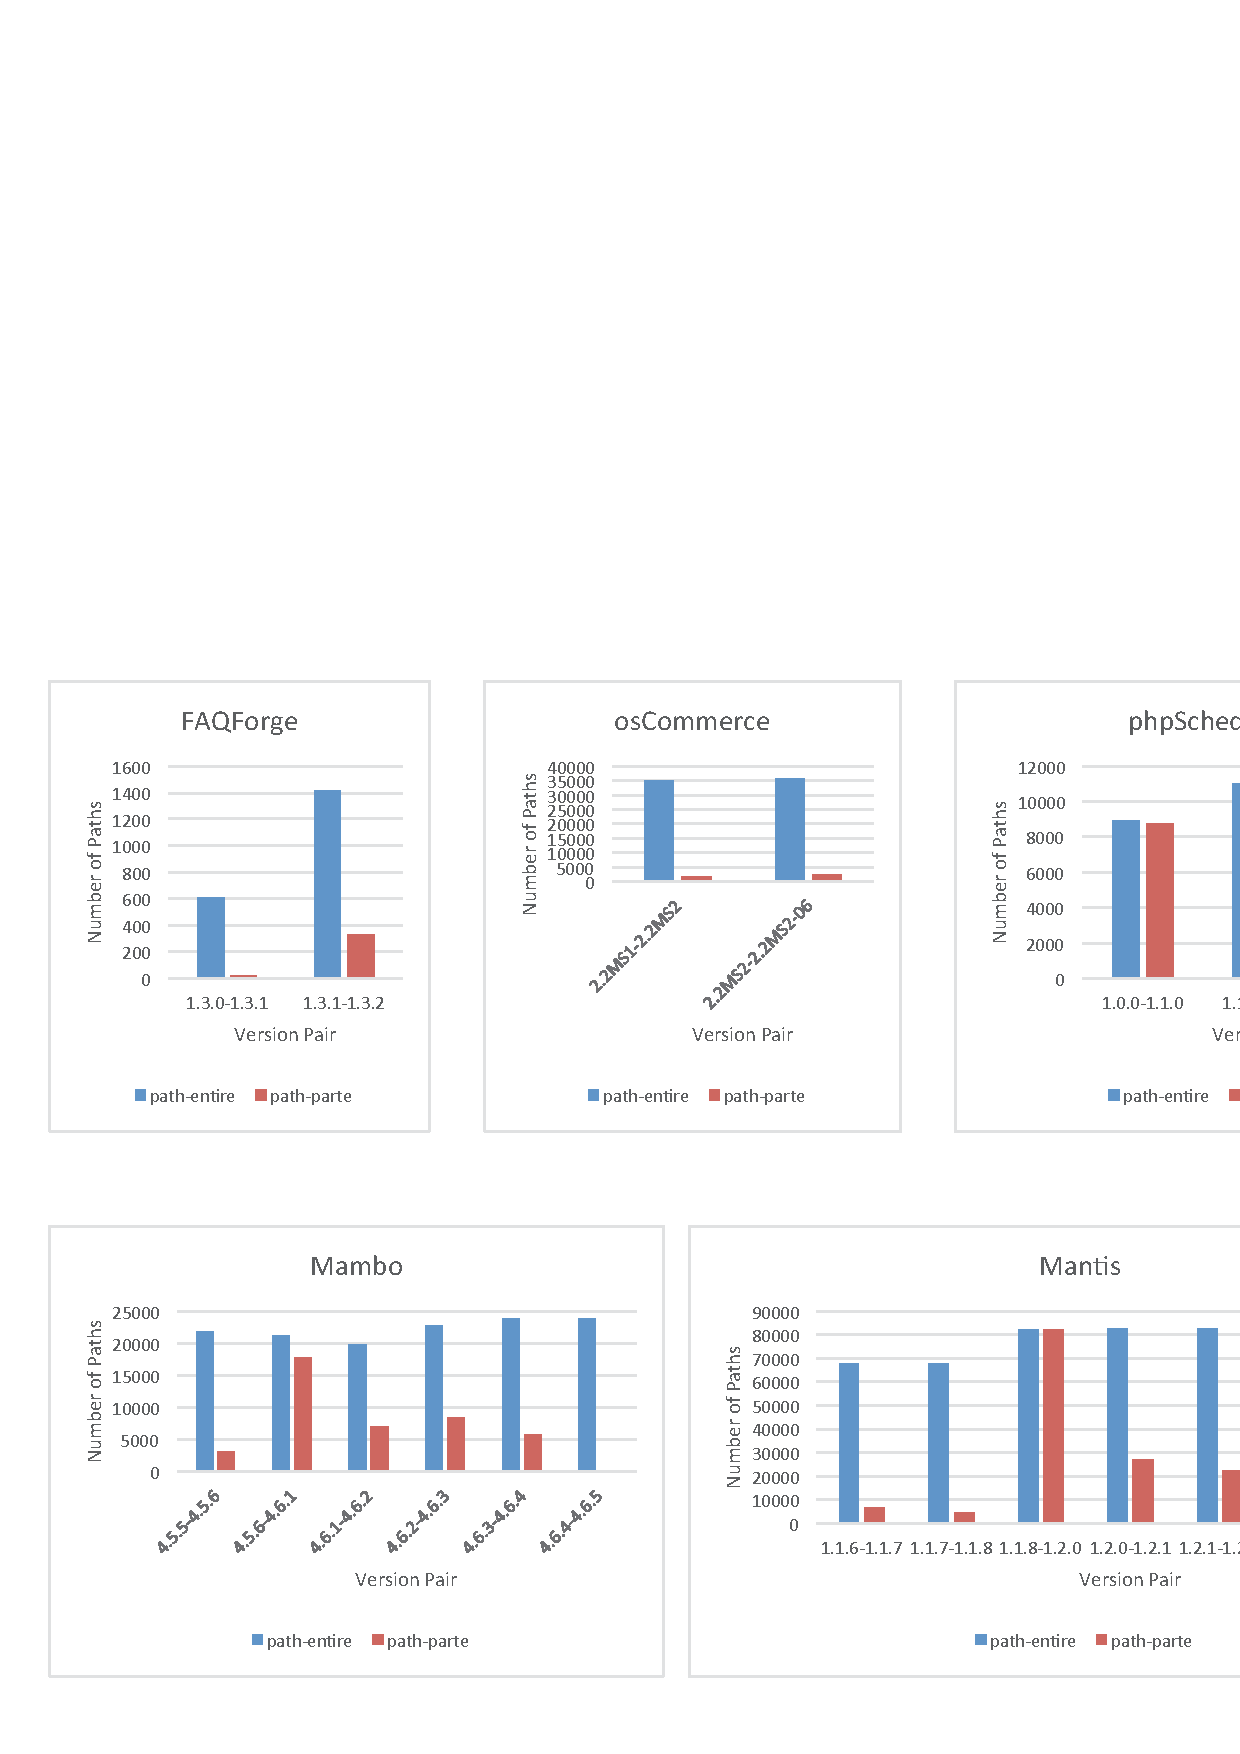
\includegraphics[width=1.0\columnwidth]{figures/bargraph.pdf}
%\leavevmode \epsfxsize=1.0\columnwidth
%\epsfbox{figures/bargraph.eps}
\vspace*{-15pt}
\caption{Experiment Results: The Total Number of Test Paths
Generated by Control and PARTE techniques}
\vspace*{5pt}
\label{fig:bargraph}
\vspace*{5pt}
\end{figure*}

\subsection{Test Input Constraints}

Because the test paths require actual inputs to create executable
test cases, by reducing the number of test paths necessary with the
modified program, we expect to produce further savings for the costs
associated with collecting test input constraints and resolving
constraints.
By automating the constraint resolution process for the majority
of inputs, we could reduce a substantial amount of time and effort
for resolving constraints manually.

To provide some ideas about how much time we can save with automatic
constraint resolution, we investigated the time taken to assign
actual values to the input variables obtained by our constraint collector.
We examined two cases from {\em osCommerce} that contain multiple numeric
and string inputs. One case has 16 inputs (2 numeric and 14 string),
and the other case has 10 inputs (2 numeric and 8 string).
To resolve all input values, it took 15 and 20 minutes, 
respectively. The tester had to go through the source files and the 
application database to figure out the proper values for them.
When we applied our tool, for the entire version of {\em osCommerce},
it took less than 5 minutes.
The input values assigned by human testers could be more realistic,
but when the number of inputs is prohibitively large to be resolved 
manually, automatic resolution would be the viable solution.
Not all inputs can be resolved with the automatic resolution tool, but
still, it would provide a good baseline that testers can utilize.

\subsection{Security Implications}

There are some security implications for this approach.
Through the experiment, we observed that the applications we 
used contained many security fixes and added security features,
and we also observed that test cases generated with our approach 
could help testers verify that a security patch or fix has been 
properly implemented.

In {\em FAQForge}, there was a security patch implemented 
between versions 1.3.1 and 1.3.2. Our test generating tool 
discovered the difference and generated several test cases 
that traversed these changes. For version 1.3.1, changes 
were made to the file that contains code for a login page that 
allows the administrators to perform security associated tasks. 
The change made to this file was the introduction of an HTML meta 
tag with an http-equiv attribute. 
This allows the page to load in all major browsers. Because the 
change happens in the header, it is important to test all code 
paths for the login page such as page load, validate username 
and password, and count failed login attempts. The test paths generated 
in our experiment include all these code paths or blocks.

In {\em osCommerce}, a similar scenario occurred between versions
2.2MS1 and 2.2MS2. The developers added some security features for 
website administration. For example, features for supporting SSL 
validation and forcing cookie usage were implemented.
Another interesting security related feature was added to
version 2.2MS2. This feature allowed users to inject shell commands 
into the web server. Our tool generated several test cases that 
covered this change. 
However, without proper inputs for these test
cases, we were not able to test this security feature correctly.
Because our current constraint resolution tool does not generate 
malicious inputs, we used our previous tool~\cite{marback09} to
generate malicious inputs. With these inputs, our tool was able 
to reveal this particular security vulnerability.
In version 2.2MS2-060817, only a few minor security fixes were made. 
For example, the fix prevented a session ID from being passed in 
Tell-A-Friend E-Mails. This fix was a minor change to the statement 
that prepares the body of the email to be sent. 
Also, there was a security fix that corrected 
an SQL injection problem between versions 2.2MS2 and 2.2MS2-060817. 
Our tool was able to generate test cases
that exercised all these fixes. 

In the case of {\em phpScheduleIt}, version 1.2.0 introduced a security 
feature where application administrators can grant permissions 
to other users. These permissions provide users the access to make, 
modify, or delete an existing reservation. Also, administrators can 
remove permissions to prevent users from accessing a resource. 
The regression tests for this version should cover code that was added 
to enable user profile management. The results from our experiment show 
that the new code blocks associated with new security features and fixes 
were included in the regression test paths generated. 

In version 4.6.2 of {\em Mambo}, a security fix was introduced. 
One such fix is about the Captcha (completely automated public 
turing test to tell computers and humans apart) feature. 
If a session is not initiated, then it is regenerated, and a new 
session code is assigned to the Captcha code. 
This produces new challenge text and audio for verification. 
Given the type and location of this fix it is important to cover all 
viable paths in this code. All these code blocks were included 
in the regression paths generated in our experiment.
 
In the case of {\em Mantis}, the version pair 1.1.6 and 1.1.7
contained one security bug fix. The fix for this bug required 
changes to the files that handle logging out of the current session 
and reloading the verification page. 
These changes impacted the blocks of code that perform logout, 
initialize a new session, and validate user credentials.
Another version pair, 1.1.8 and 1.2.0, contained one security fix. 
The bug was about the possibility of a cross site scripting attack 
through permalink\_page.php. The fix was to check if the input URL 
is safe. Because this change happened at the root level, all paths 
in the permalink\_page.php file should be included to test the fix,
and our tool was able to generate those paths. 
 
\subsection{Limitations}
\label{sec:limitations}

Although our approach and empirical results are promising,
our approach has some limitations that we want to address. 
One limitation involves test oracles. As we mentioned
in Section~\ref{sec:method}, in this work, we focused
on generating test cases, and our approach does not generate
the oracles. Automating test oracle generation or verification 
of the results could be investigated in the future. 
 
Another limitation involves test case execution.
To execute test cases automatically, the test execution engine 
needs to pass the web elements to Selenium along with test paths and
input values. However, the current path generator does not 
provide web elements, so we had to provide them manually.
As a result, we were not able to run all test cases that 
we generated through our tool. However, this issue has been identified,
and the feature addition is being developed. 
 

\section{Threats to Validity}
\label{sec:validity}

The primary threat to validity of this study is the amount of
user session data and the type of users who participated in this
study. For the private application that we used in this study,
we collected user interaction data for a long period time; 
the collected data was created by actual users of 
the application. However, for the two open source applications, 
the period of time that we collected user interactions was relatively 
short, and the participants were not domain experts or regular users 
of the applications so their usage patterns had wide variations.
This threat can be addressed by performing additional studies that
monitor user interactions over a longer time period among a wider population,
by considering industrial applications and different types of 
applications (e.g., mobile applications).
 
Another threat to validity is the choice of algorithms that classify 
components' frequency access ranking and analyze change impact. 
In this study, we applied various algorithms to create our classification
model, but many other classification algorithms (e.g., decision tree and
apriori algorithms) are available, and they could produce different results.
The results can vary depending on the type of classification algorithms, 
the parameters set for classification algorithms, the variables being analyzed, 
and the environmental settings. 

There is another concern regarding the bug reports that we used.
Our classification prediction values for designing linear models 
in the change impact analysis were generated from bug history that 
was reported by actual users.
Further, using these bug reports, we measured the coefficient of other 
variables to create our linear model for change impact analysis.
Because our bug report data is not comprehensive and contains 
only those bugs accrued 
until the time that we stopped collecting data, 
and because there might 
be other bugs that have not been reported yet or that might occur 
later, there is a possibility that the bug reports are biased.


%In this section, we describe the internal and external
%threats to the validity of our study. We also describe 
%the approaches we used to limit the effects of these threats.
%
%{\em Internal Validity:}
%The outcome of our study could be affected by the choice of 
%program analysis. We applied static analysis on a dynamic programming 
%language, PHP. To do so, we had to change many statements in the 
%program during the file preparation phase, removing and fixing 
%many dynamic environment variables. However, we carefully examined 
%our process to minimize the adversary effect that might be introduced
%into the converted files.  
%
%{\em External Validity.}
%We used open source web applications for our study, so these programs 
%are not representative of the applications used in practice, and thus
%we cannot generalize our results. However, we tried to reduce this 
%threat by using five non-trivial sized web applications with multiple 
%versions that have been utilized by many users. 


\vspace*{2pt}
\section{Related Work}
\label{sec:related-work}

This section discusses two topics related to our research:
test case prioritization techniques and recommender systems.

\subsubsection*{Test Case Prioritization}
%Test case prioritization techniques reorder test cases to maximize
%some objective functions, such as detecting defects as early as possible.
Due to the appealing benefits of test case prioritization in practice, 
many researchers have proposed various  
techniques.These techniques help engineers discover faults
early in testing, which allows them to begin debugging earlier.
%In this case, entire test suites may still be executed, which avoids 
%the potential drawbacks associated with omitting test cases. 
Recent surveys ~\cite{catal13, marksurvey} provide a comprehensive 
understanding of overall trends of the techniques and suggest areas for improvement.
Depending on the types of information available, various test case
prioritization techniques can be utilized, but 
the majority of prioritization techniques have used source code
information to implement the techniques.
For instance, many researchers have utilized code coverage information
to implement prioritization techniques~\cite{elbaum02feb, kim02may,rothermel01oct}. 
Although this approach is na\"{\i}ve, many empirical
studies have shown that this approach can be effective~\cite{cost3, 
cost1, Malishevsky02, myra}.
%Recent prioritization techniques have used other
%types of code information, such as slices~\cite{jeffrey06sep}, change
%history~\cite{sherriff07}, code modification information, and fault
%proneness of code~\cite{mirarab07}.

Further, some researchers have used software risk information in testing approaches.  
For instance, Frankl and Weyuker ~\cite{weyuker} introduced two risk related measures of 
software testing effectiveness, which are expected detected risk and expected risk reduction
and investigated the effectiveness of these two measures on testing techniques. 
%Chen et al.~\cite{chenRisk} presented a black box
%regression test selection technique, which is a customer-oriented
%and risk-based.
Hettiarachchi et al.~\cite{risk} proposed a new test case
prioritization technique. Their technique uses risk levels of potential defects
to detect risky requirements then it prioritizes test cases by mapping the related 
test cases and these requirements.

More recently, several prioritization techniques 
utilizing other types of information have also been proposed. 
For example, Anderson et al. applied telemetry data to compute fingerprints 
to extract usage patterns and for test prioritization~\cite{jeff16}.
Memon and Amalfitano performed a study applying telemetry 
data to generate usage pattern profiles~\cite{memongui}.  
%In another study, Amalfitano et al. built finite state models
%based on usage data that they collected from rich Internet applications ~\cite{rich}. 
%Carlson et al.~\cite{ryan} presented clustering-based techniques that
%utilize real fault history information including code coverage.
%Anderson et al.~\cite{jeff14} investigated the use of various code features
%mined from a large software repository to improve regression testing techniques.
Gethers et al. presented a method  that uses textual change of source code
to estimate an impact set ~\cite{kagdichange}. 

\subsubsection*{Recommender Systems}  
Recommender systems are software engineering tools that make 
the decision making process easier by providing a list of relevant items.
%There are three primary  categories in recommender systems:
%content-based algorithms, collaborative filtering algorithms, 
%and hybrid approaches ~\cite{recomsurvey05}.  
%Recommender systems are commonly used by users in their daily routines, 
%helping in such tasks as finding 
%their target items more easily.
Some widely-used applications that provide recommender systems
are Amazon, Facebook, and Netflix. These applications provide suggestions
to target users based on the user or on item characteristic similarities.  

%Further, in the area of software engineering, due to the decline in hardware 
%facility prices, a variety of information is collected by software 
%providers, such as change history, issue reports and databases, user log files, 
%and so on.
With the fast growth of such information, machine learning technologies  
motivate software engineers to apply recommendation systems in software 
development. Recommender systems in software engineering have been applied  
to improve software quality and to address the challenges of the development process~\cite{rssebook}.  
For instance, Murakami et al. ~\cite{murakami} proposed a technique that 
uses user editing activities  detecting code relevant to existing methods. 
%Christidis et al. ~\cite{costas} implemented a recommender system 
%to display developer activities by using information artifacts with quantitative metrics. 
Danylenko and Lowe provided a context-aware recommender system 
to automate a decision-making process for determining the efficiency of 
non-functional requirements ~\cite{contextawar}.

As discussed briefly earlier, many types of information are available 
for implementing test case prioritization techniques.
In this research, we collected over 2,000 user sessions from 
three different web applications and gathered the change history of each application. 
Our research seeks to apply item-based collaborative filtering algorithms 
to generate a recommendation list for test prioritization.
To our knowledge, our recommender system-based prioritization technique is novel 
and has not yet been explored in regression testing.



\section{Conclusions and Future Work}
\label{sec:conclusions}

In this research, we proposed a new recommender system to 
improve the effectiveness of test case prioritization. 
Our recommender system uses three datasets (code coverage, change history, and user sessions)
to produce a list of most risky components of a system for regression testing.
We applied our recommender system using two open source applications and 
one industrial application to investigate whether our approach 
can be effective compared to four different control techniques.
The results of our study indicate that our recommender system can help 
improve test prioritization; also, the performance of our approach 
was particularly noteworthy  outstanding when we had a limited time budget. 

Because our initial attempt to use recommender systems in the area of regression 
testing showed promising results, we plan to investigate this approach further
by considering various algorithms (e.g., a context-aware algorithm and a hybrid algorithm), 
the characteristics of applications, and the testing context.
For example, as we discussed earlier, there are some limitations in collaborative 
filtering. In future research, we plan to investigate other approaches 
to address a sparsity problem by applying an associative
retrieval framework and related spreading activation algorithms
to track user transitive interactions through their previous interactions. 
Also, to address the ``New Item Problem,'' we plan to apply 
knowledge-based techniques such as case-based reasoning. 
Further, in this study, we did not evaluate our approach considering
cost-benefit tradeoffs, so we would like to investigate this aspect in a future study. 
Also, we wish to apply our recommender system to different software domains 
such as mobile applications and perform additional studies that
monitor user interactions over a longer period of time.


%
\subsection*{Acknowledgments}

This work was supported, in part, by NSF CAREER Award
CCF-1564238 to University of North Texas.



%\balance
\bibliographystyle{plain}
\bibliography{paper}

\end{document}
